\chapter{Product Design}
\section{Wireless Personal Area Network}
WPAN \textbf{(wireless personal area network)} is a personal area network- a network for interconnecting devices centered around an individual person's workspace in which the connections are wireless. Typically, a wireless personal area network uses some technology that permits communication within about 10 meters - in other words, a very short range.\\
Wireless PAN is based on the standard \textbf{IEEE 802.15.4}. A WPAN could serve to interconnect all the ordinary computing and communicating devices that many people have on their desk or carry with them today; or it could serve a more specialized purpose such as allowing the surgeon and other team members to communicate during an operation. There are also many other existing standard such as the IEEE802.11 which is the (wireless local area network) wlan so why there is a need to developed the new standards so the answer is simple that it requires less power, lesser  bandwidth, has low penetration.
\subsection{Limitations}
WPAN has been designed with some specific fundamentals that happen to serve in a lot of application fields. But this does not means  that it is not apt other kind of applications. Most of its limitations are due to the following two fundamental fact
\begin{enumerate}
	\item The maximum therotical throughput is i\textbf{500Kbps} which is reduces by several factors to only \textbf{5-10KBps} in most cases.
	\item The operating range is generally \textbf{2-5 meters}. This can be extended to \textbf{30 meters} or so but that will of course demand higher strain on the battery life of the devices. This is the defining thing about the BLE technology that the devices are mostly passive in nature and hence it becomes very important for them to have large battery life. In some cases it is seen that the device’s battery can actually outlast other hardware in the device itself.
	\item The loss of the data in Wlan goes upto \textbf{60} which is much higher than that of the wpan ahich have only \textbf{30} data loss.
	\item Frankly speaking, there is no much benefits of Wireless personal area network over wireless local area network \textbf{WLAN}the wlan consumes more power because it transmits the data for a longer distance and have the throughput upto 10Mbps. Wpan useful for the short distance communication and low data transmission.
\end{enumerate}
\subsection{WPAN Architecture}
\subsubsection{Application layer}  The upper layer containing most of the application logic, that is used to transfer the data. 6lowpan is the mostly used upper layer.
\subsubsection{Host} It Contains all the lower layer protocols like PHY and MAC layer in WPAN IEEE802.15.4 acts as the host.
\subsubsection{Controller}  Linux acts as the controller for wpan.
We will discuseed all these layer one by one so first we start with host because it acts on the ground means it contains the RF layer.
\subsection{IEEE 802.15.4 Network Topologies}
Network topology defines the way in which different devices (under different roles) interact with one another to exchange data through transceiver. These topologies are defined under the specification and are maintained under the IEEE guidelines.\\
Depending on the application requirements, an IEEE 802.15.4 LR-WPAN operates in either of two topologies:
\begin{enumerate}
	\item Star topology.
	\item Peer to Peer topology.
\end{enumerate}
Let's take a look ate each of them individually.
\subsubsection{Star Topology}
In the star topology, the communication is established between devices and a single central controller, called the PAN coordinator. A device typically has some associated application and is either the initiation point or the termination point for network communications. A PAN coordinator can also have a specific application, but it can be used to initiate, terminate, or route communication around the network. The PAN coordinator is the primary controller of the PAN
All devices operating on a network of either topology have unique addresses referred to as extended addresses we will discussed it later that what is extended address. A device will use either the extended address for direct communication within the PAN or the short address that was allocated by the PAN coordinator when the device associated. The PAN coordinator will often be mains powered, while the devices will most likely be battery powered. Applications that benefit from a star topology include home automation, personal computer (PC) peripherals, games, and personal health care.
\begin{figure}[ht]
	\centering
	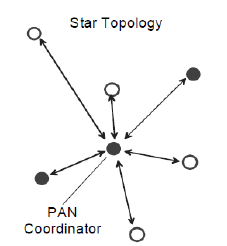
\includegraphics[scale=1.2]{images/star_topology.png}
	\caption{Star topology}
\end{figure}
\subsubsection{Peer to Peer Topology}
The peer-to-peer topology also has a PAN coordinator; however, it differs from the star topology in that any device is able to communicate with any other device as long as they are in range of one another. Peer-to-peer topology allows more complex network formations to be implemented, such as mesh networking topology. Applications such as industrial control and monitoring, wireless sensor networks, asset and inventory tracking, intelligent agriculture, and security would benefit from such a network topology. A peer-to-peer network allows multiple hops to route messages from any device to any other device on the network. Such functions can be added at the higher layer, but they are not part of this standard. Each independent PAN selects a unique identifier. This PAN identifier allows communication between devices within a network using short addresses and enables transmissions between devices across independent networks. The mechanism by which identifiers are chosen is outside the scope of this standard.
\begin{figure}[ht]
	\centering
	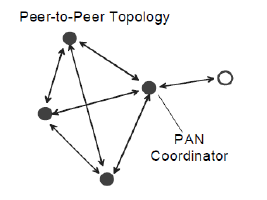
\includegraphics[scale=1]{images/peertopeertopology.png}
	\caption{Peer to Peer topology}
\end{figure}
\subsection{Network formation}
\subsubsection{Star network formation}
After an FFD is activated, it can establish its own network and become the PAN coordinator. All-star networks operate independently from all other star networks currently in operation. This is achieved by choosing a PAN identifier that is not currently used by any other network within the radio communications range. Once the PAN identifier is chosen, the PAN coordinator allows other devices, potentially both FFDs and RFDs, to join its network.
\subsubsection{Peer to Peer network formation}
In a peer-to-peer topology, each device is capable of communicating with any other device within its radio communications range. One device is nominated as the PAN coordinator, for instance, by virtue of being the first device to communicate on the channel. Further network structures are constructed out of the peer-to peer topology, and it is possible to impose topological restrictions on the formation of the network.\\
An example of the use of the peer-to-peer communications topology is the \textbf{cluster tree}. The cluster tree network is a special case of a peer-to-peer network in which most devices are FFDs. An RFD connects to a cluster tree network as a leaf device at the end of a branch because RFDs do not allow other devices to associate. Any FFD is able to act as a coordinator and provide synchronization services to other devices or other coordinators. Only one of these coordinators is the overall PAN coordinator, potentially because it has greater computational resources than any other device in the PAN. The PAN coordinator forms the first cluster by choosing an unused PAN Identifier and broadcasting beacon frames to neighbouring devices.
\begin{figure}[ht]
	\centering
	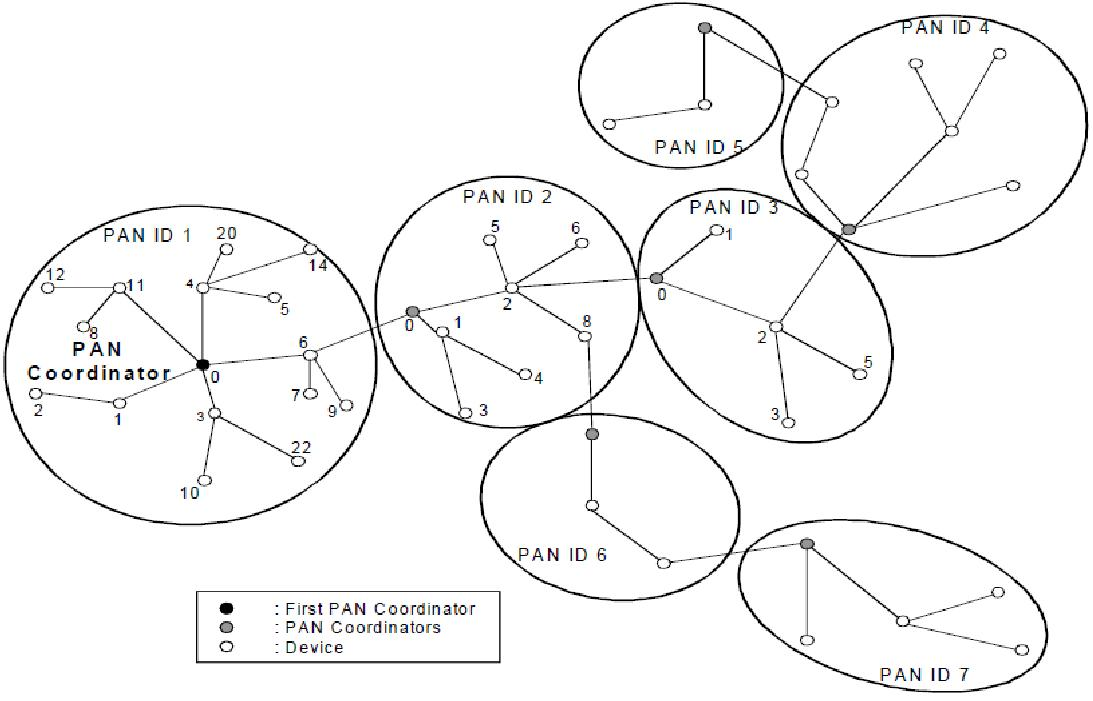
\includegraphics[scale=0.4]{images/cluster_tree.png}
	\caption{Cluster network}
\end{figure}
\section{IEEE 802.15.4 Architecture}
The IEEE 802.15.4 architecture is defined in terms of a number of blocks in order to simplify the standard. These blocks are called layers. Each layer is responsible for one part of the standard and offers services to the higher layers. As OSI have 7 layer but the IEEE 802.1.5.4 constitutes only the lower two layer\\
\begin{enumerate}

	\item{Physical layer(PHY)}
	\item{Medium access control(MAC) layer}
\end{enumerate}
	An LR-WPAN device comprises at least one PHY, which contains the radio frequency (RF) transceiver along with its low-level control mechanism, and a MAC sublayer that provides access to the physical channel for all types of transfer.



\begin{figure}[ht]
	\centering
	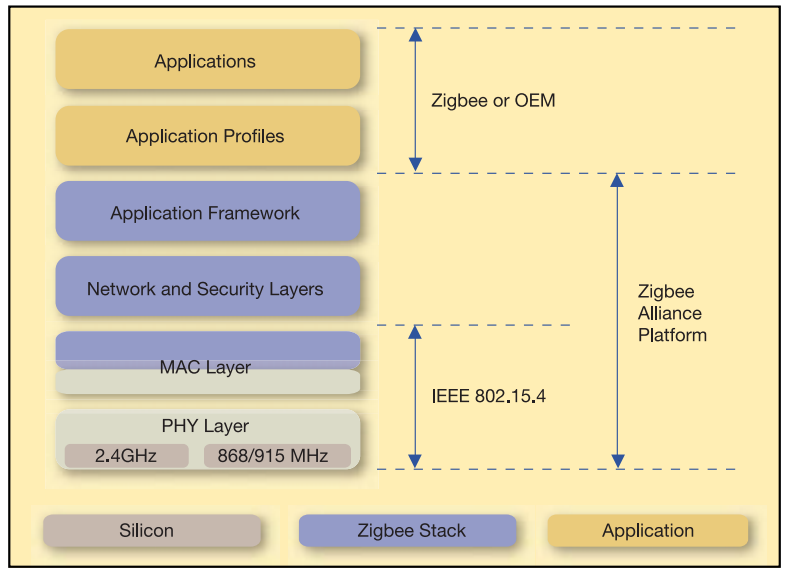
\includegraphics[scale=0.7]{images/ieee.png}
	\caption{IEEE 802.15.4}
\end{figure}
The upper layers, shown in figure, consist of a network layer, which provides network configuration, manipulation, and message routing, and an application layer, which provides the intended function of the device. The upper layer covered by the 6lowpan. We will discussed the upper layers function in the coming chapter.
\subsection{Physical layer}
The physical layer is the first layer of the Open System Interconnection Model (OSI Model). The physical layer deals with bit-level transmission between different devices and supports electrical or mechanical interfaces connecting to the physical medium for synchronized communication.\\
The PHY is responsible for the following tasks:\\
\begin{enumerate}
	\item{Activation and deactivation of the radio transceiver}
	\item {Energy detection (ED) within the current channel}
	\item {Link quality indicator (LQI) for received packets}
	\item {Clear channel assessment (CCA) for carrier sense multiple access with collision avoidance\textbf{(CSMA/CA)}}
	\item {Channel frequency selection}
	\item{Data transmission and reception}
	\item{Precision ranging for ultra-wide band\textbf{(UWB)}PHY's}
\end{enumerate}
The PHYs defined in this standard are:\\
O-QPSK PHY: \\Direct sequence spread spectrum (DSSS) PHY employing offset quadrature phase shift keying (O-QPSK) modulation, operating in the 780 MHz bands, 868 MHz, 915 MHz, and 2450 MHz.\\
BPSK PHY: \\DSSS PHY employing binary phase-shift keying (BPSK) modulation, operating in the 868 MHz, 915 MHz, and 950 MHz bands.\\
ASK PHY: \\Parallel sequence spread spectrum (PSSS) PHY employing amplitude shift keying.\\
ASK and BPSK modulation, operating in the 868 MHz and 915 MHz bands.\\
CSS PHY: \\Chirp spread spectrum (CSS) employing differential quadrature phase-shift keying.\\
DQPSK:\\  DQPSK modulation, operating in the 2450 MHz band.\\
UWB PHY: \\Combined burst position modulation (BPM) and BPSK modulation, operating in the sub-gigahertz and 3–10 GHz bands.\\
MPSK PHY: \\M-ary phase-shift keying (MPSK) modulation, operating in the 780 MHz.\\
GFSK PHY: \\Gaussian frequency-shift keying (GFSK), operating in the 950 MHz band.\\
\subsection{Operating frequency range}
A compliant device shall operate in one or several frequency bands using the modulation and spreading formats. Devices shall start in the PHY mode in which they are instructed to start. If the device is capable of operating in the 868 MHz or 915 MHz bands using one of the optional PHYs and, it shall be able to switch dynamically between the optional PHY and the mandatory BPSK PHY in that band when instructed to do so. If the 950 MHz band is supported, then at least one of the 950 MHz band PHYs shall be implemented.
\subsection{Medium Acess Control}
The Media Access Control Layer is one of two sublayers that make up the Data Link Layer of the OSI model sublayer handles all access to the physical radio channel and is responsible for the following tasks:
\begin{enumerate}
	\item{Generating network beacons if the device is a coordinator}
	\item{Synchronizing to network beacons}
	\item{Supporting PAN association and disassociation}
	\item{Supporting device security}
	\item{Employing the CSMA-CA mechanism for channel access}
	\item{Handling and maintaining the GTS mechanism}
	\item{Providing a reliable link between two peer MAC entities}
\end{enumerate}
There are two device types:\\ 
Full-function device (FFD)\\ 
Reduced-function device (RFD)\\ 
The FFD may operate in three modes serving as a personal area network (PAN) coordinator, a coordinator, or a device. An RFD shall only operate as a device.
\subsubsection{MAC Services}
The MAC sublayer provides an interface between the next higher layer and the PHY. The MAC sublayer conceptually includes a management entity called the mac layer management activity (MLME). This entity provides the service interfaces through which layer managementons may be invoked. The MLME is also responsible for maintaining a database of managed objects pertaining to the MAC sublayer. This database is referred to as the MAC sublayer PIB.
\begin{figure}[ht]
	\centering
	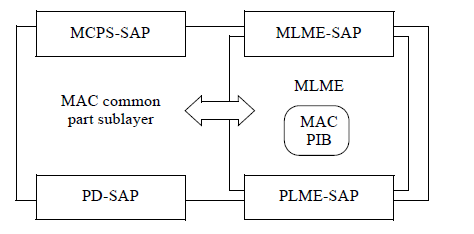
\includegraphics[scale=1]{images/macsublayer.png}
	\caption{MAC Sublayer reference model}
\end{figure}
\subsection{Security}
The MAC sublayer is responsible for providing security services on specified incoming and outgoing frames when requested to do so by the higher layers. The 802.15.4 standard supports the following security services:
\begin{enumerate}
	\item{Data confidentiality}
	\item{Data authenticity}
	\item{Replay protection}
\end{enumerate}
A device may optionally implement security. A device that does not implement security shall not provide a mechanism for the MAC sublayer to perform any cryptographic transformation on incoming and outgoing frames nor require any PIB attributes associated with security. A device that implements security shall provide a mechanism for the MAC sublayer to provide cryptographic transformations on incoming and outgoing frames using information in the PIB attributes associated with security only if the macSecurityEnabled attribute is set to TRUE.\\
\subsection{MAC layer advertising and scanning}
The advertising packets are used to either broadcast data for applications or to discover slaves and to connect to them. The advertising of packets is done aftmake a entry for SPIRIT in sysfs.er certain intervals and if during this interval some device is scanning then that device will be able to receive the advertising packet.\\
The advertising packets are used to either broadcast data for applications or to discover slaves and to connect to them. The advertising of packets is done after make a entry for SPIRIT in sysfs after certain intervals and if during this interval some device is scanning then that device will be able to receive the advertising packet.\\
The specification defines the two types of scanning\\
\subsubsection{Passive Scanning}
The scanner simply listens for advertising packets, and the advertiser is never aware of the fact that one or more packets were actually received by a scanner.
\subsubsection{Active Scanning}
The scanner issues s Scan Request packet after receiving an advertising packet. The advertiser receives it and responds with a Scan Response packet. This additional packet doubles the effective payload that the advertiser is able to send to the scanner, but it is important to note that this does not provide a means for the scanner to send any user data at all to the advertiser.\\
Before commencing an active or passive scan, the MAC sublayer shall store the value of macPANId and then set it to 0xffff for the duration of the scan this enables the receive filter to accept all beacons. On completion of the scan, the MAC sublayer shall restore the value of macPANId to the value stored before the scan began.
\section{Low Wireless Personal Area Network}
The 6LoWPAN group has defined encapsulation and header compression mechanisms that allow IPv6 packets to be sent and received over IEEE 802.15.4 based networks. IPv4 and IPv6 are the work horses for data delivery for local-area networks, metropolitan area networks, and wide-area networks such as the Internet. Likewise, IEEE 802.15.4 devices provide sensing communication-ability in the wireless domain. The inherent natures of the two networks though, are different.
\subsection{Transmission of IPv6 Packets over IEEE 802.15.4 Networks}
The 6lowpan sits over the IEEE802.15.4 packets, which acts as the convergence layer for the packet transmission.
\begin{figure}[ht]
	\centering
	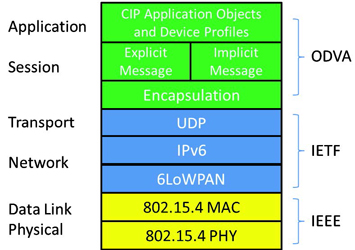
\includegraphics[scale=1]{images/6lowpan.png}
	\caption{6 Lowpan over IEEE}
\end{figure}
\subsection{IEEE 802.15.4 Mode over IPv6} 
IEEE 802.15.4 defines four types of frames\\
\begin{enumerate}
	\item{Beacon frames}
	\item{MAC command frames}
	\item{Acknowledgement frames}
	\item{Data frames}
\end{enumerate}
IPv6 packets MUST be carried on data frames. Data frames may optionally request that they be acknowledged. IEEE 802.15.4 networks can either be nonbeacon-enabled or beacon-enabled.  The latter is an optional mode in which devices are synchronized by a so-called coordinator's beacons.  This allows the use of superframes within which a contention-free Guaranteed Time Service (GTS) is possible. In nonbeacon-enabled networks, data frames (including those carrying IPv6 packets) are sent via the contention-based channel access method of unslotted CSMA/CA. In nonbeacon-enabled networks, beacons are not used for synchronization. However, they are still useful for link-layer device discovery to aid in association and disassociation events.
\subsection{Addressing Modes}
IEEE 802.15.4 defines several addressing modes, it allows the use of either:\\
1. IEEE 64-bit extended addresses or (after an association event)\\
2. 16-bit addresses unique within the PAN.\\
6lowpan supports both the addresses. Short addresses being transient in nature, a word of caution is in order. Since they are doled out by the PAN coordinator function during an association event, their validity and uniqueness is limited by the lifetime of that association.
\subsection{Maximum transmission Unit}
The MTU size for IPv6 packets over IEEE 802.15.4 is 1280 octets. However, a full IPv6 packet does not fit in an IEEE 802.15.4 frame. 802.15.4 protocol data units have different sizes depending on how much overhead is present.  Starting from a maximum physical layer packet size of 127 octets (aMaxPHYPacketSize) and a maximum frame overhead of 25 (aMaxFrameOverhead), the resultant maximum frame size at the media access control layer is 102 octets. Link-layer security imposes further overhead, which in the maximum case (21 octets of overhead in the AES-CCM-128 case, versus 9 and 13 for AES-CCM-32 and AES-CCM-64, respectively) leaves only 81 octets available.  This is obviously far below the minimum IPv6 packet size of 1280 octets. Furthermore, since the IPv6 header is 40 octets long, this leaves only 41 octets for upper-layer protocols, like UDP.  The latter uses 8 octets in the header which leaves only 33 octets for application data.  Additionally, there is a need for a fragmentation and reassembly layer, which will use even more octets.\\
\begin{enumerate}
	\item{The adaptation layer must be provided to comply with the IPv6 requirements of a minimum MTU.  However, it is expected that}
	\begin{itemize}
		\item Most applications of IEEE 802.15.4 will not use such large packets.
		\item Small application payloads in conjunction with the proper header compression will produce packets that fit within a single IEEE 802.15.4 frame.  The justification for this adaptation layer is not just for IPv6 compliance, as it is quite likely that the packet sizes produced by certain application exchanges (e.g., configuration or provisioning) may require a small number of fragments.
		\end{itemize}
	\item{Even though the above space calculation shows the worst-case scenario, it does point out the fact that header compression is compelling to the point of almost being unavoidable.  Since we expect that most (if not all) applications of IP over IEEE 802.15.4 will make use of header compression.}
\end{enumerate}
\begin{figure}[ht]
	\centering
	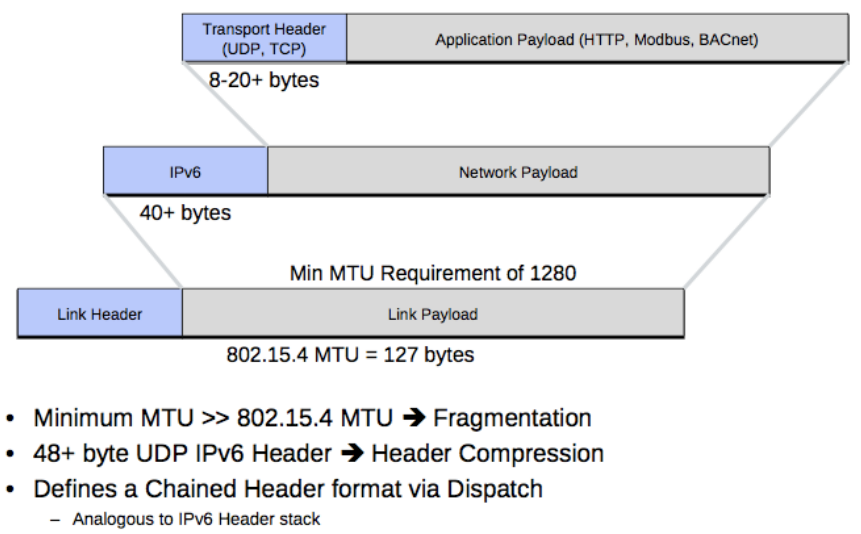
\includegraphics[scale=0.51]{images/headercompression.png}
	\caption{Fragmentation and defragmentation}
\end{figure}
\subsection{Security of IPv6}
The method of derivation of Interface Identifiers from EUI-64 MAC addresses is intended to preserve global uniqueness when possible. However, there is no protection from duplication through accident or forgery. Neighbor Discovery in IEEE 802.15.4 links may be susceptible to threats.  Mesh routing is expected to be common in IEEE 802.15.4 networks. This implies additional threats due to ad hoc routing.  IEEE 802.15.4 provides some capability for link-layer security. Users are urged to make use of such provisions if at all possible and practical.  Doing so will alleviate the threats stated above. \\A sizeable portion of IEEE 802.15.4 devices is expected to always communicate within their PAN (i.e., within their link, in IPv6 terms).  In response to cost and power consumption considerations, and in keeping with the IEEE 802.15.4 model of "Reduced Function Devices" (RFDs), these devices will typically implement the minimum set of features necessary.  Accordingly, security for such devices may rely quite strongly on the mechanisms defined at the link layer by IEEE 802.15.4.  The latter, however, only defines the Advanced Encryption Standard (AES) modes for authentication or encryption of IEEE 802.15.4 frames, and does not, in particular, specify key management (presumably group oriented).  Other issues to address in real deployments relate to secure configuration and management. Whereas such a complete picture is out of the scope of this document, it is imperative that IEEE 802.15.4 networks be deployed with such  considerations in mind.  Of course, it is also expected that some IEEE 802.15.4 devices (the so-called "Full Function Devices", or "FFDs") will implement coordination or integration functions.  These may communicate regularly with off-link IPv6 peers (in addition to the more common on-link exchanges).  Such IPv6 devices are expected to secure their end-to-end communications with the usual mechanisms (e.g., IPsec, TLS, etc).
\section{WPAN The officila Linux SPIRIT stack}
\textbf{WPAN}is the official Linux personal area protocol stack. It is an Open Source project distributed under the GNU General Public License (GPL).
\begin{figure}[ht]
	\centering
	
\includegraphics[scale=1]{images/linux.png}
	\caption{WPAN the officila SPIRIT stack of Linux}
\end{figure}
\subsection{History}
The linux-wpan project was started in 2008. Initially, it was started with the name of linux-zigbee but this name is little confusing because there is no zigbee protocol at all and  linux is an open source wheras zigbee is managed by zigbee community. The lower layer consist of the PHY and MAC layer as we discussed above and the transport layer consist of the Zigbee protocol.
\begin{figure}[ht]
	\centering
	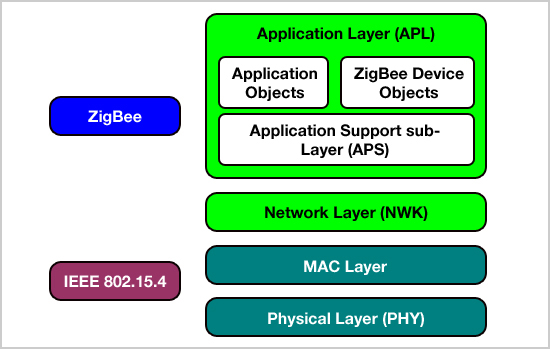
\includegraphics[scale=0.8]{images/wpan.png}
	\caption{Linux-WPAN}
\end{figure}
Mainly Community slowly took over and the new open standard was formed to avoid confusion with the name linux-wpan and the new maintainer were Alexander Aring and Pengutronix. Now there are many higher layer protocols which make the use of IEEE 802.15.4 profiles.\\
These are discussed below:\\
\begin{enumerate}
	\item{Zigbee}
	\begin{itemize}
		\item Zigbee Alliance's mesh networking protocol but it’s not available under the GPL licensing as we discussed above.
	\item{MiWi Mesh and MiWi P2P}
		\item Microchip's proprietary mesh and P2P protocols. This protocol is only compatible with the Microchip’s component and they have their own standard.
	\item{6LoWPAN}
		\item IPv6 over 802.15.4.
	\item{WirelessHART}
		\item It’s mainly used for Industrial Automation purpose because it required the more power and data sent by this protocol is of higher bits.
	\end{itemize}
\end{enumerate}
So we have only one option left i.e. IPv6 over 802.15.4.\\
But many of the protocols of the linux-WPAN is taken from the linux-WLAN. If we compare both of the frameworks then.\\ \\
\begin{table}[ht]
	\centering
	\scalebox{1.2}{
	\begin{tabular}{|K{2.2cm} | K{8cm} | K{2.2cm}|}
		\toprule
		\rowcolor{Gray}
		\textbf{wpan} & \textbf{Description} & \textbf{wlan} \\
		\hline
		wlan & Default interfacing naming & wpan \\
		\hline
		station & Default interfacing type registration & node \\
		\hline
		iw & command framework & iwpan \\
		\hline
		nl80211 & Netlink kernel framework & nl802154 \\
		\hline
		cfg80211 & Soft and Hard-MAC Interface & cfg802154 \\
		\bottomrule
	\end{tabular}}
	\caption{wlan and wpan framework}
\end{table}
\section{SPIRIT2}
The S2-LP is a narrow band ultra-low power RF transceiver, intended for RF wireless applications in the sub-1 GHz band. It is designed to operate in both the license-free ISM and SRD frequency bands at 433,868 and 920 MHz, but can also be programmed to operate at other additional frequencies in the 430-470 MHz, 860-940 MHz bands. The S2-LP supports different modulation schemes: 2(G)FSK, 4(G)FSK, OOK and ASK. The air data rate is programmable from 0.3 to 500 kbps. The S2-LP can be used in systems with channel spacing of 12.5/25 kHz, complying with the EN 300 220 standard and satisfying the latest FCC narrow banding mandate.
The S2-LP shows a RF link budget higher than 140dB for long communication range and meets the regulatory requirements applicable in territories worldwide, including Europe, Japan, China and USA. The S2-LP integrates a configurable baseband modem with proprietary fully programmable packet format allowing also:
\begin{enumerate}
	\item{IEEE 802.15.4g full hardware packet supporting whitening, CRC, FEC and dual SYNC
	word detection.}
	\item{Wireless M-Bus standard compliance packet format (all performance classes).
	In order to reduce the overall system power consumption and increase the communication reliability, the S2-LP provides an embedded programmable automatic packet acknowledgment, automatic packet retransmission, CSMA/CA engine, low duty cycle protocol, RX sniff mode and timeout protocol. The S2-LP fully supports antenna diversity with an integrated antenna switching control algorithm. Transmitted/received data bytes are buffered in two different 128 bytes FIFOs (TX FIFO and RX FIFO), accessible via SPI interface for host processing. In addition the reduction of external components enables easily and fast integrate the S2-LP on products to enable a short time to market.}
\end{enumerate}
\subsection{Block diagram of SPIRIT2}
The receiver architecture is low-IF conversion, the received RF signal is amplified by a two-stage lownoise amplifier (LNA) and down-converted in quadrature (I and Q) to the intermediate frequency (IF). LNA and IF amplifiers make up the RX front-end (RXFE) and have programmable gain. The transmitter part of the S2-LP is based on direct synthesis of the RF frequency. The power amplifier (PA) input is the LO generated by the RF synthesizer, while the output level can be configured between -30 dBm and +14 dBm (+16 dBm in boost mode), at pin level with 0.5 dB steps. The data to be transmitted can be provided by an external MCU either through the 128-byte TX FIFO writable via SPI, or directly using a programmable GPIO pin.\\
The S2-LP supports frequency hopping, TX/RX and antenna diversity switch control, extending the link range and improving performance. The S2-LP has a very efficient power management (PM) system. An integrated switched mode power supply (SMPS) regulator allows operation from a battery voltage ranging from +1.8 V to +3.6 V, and with power conversion efficiency of 90percent.
\begin{figure}[ht]
	\centering
	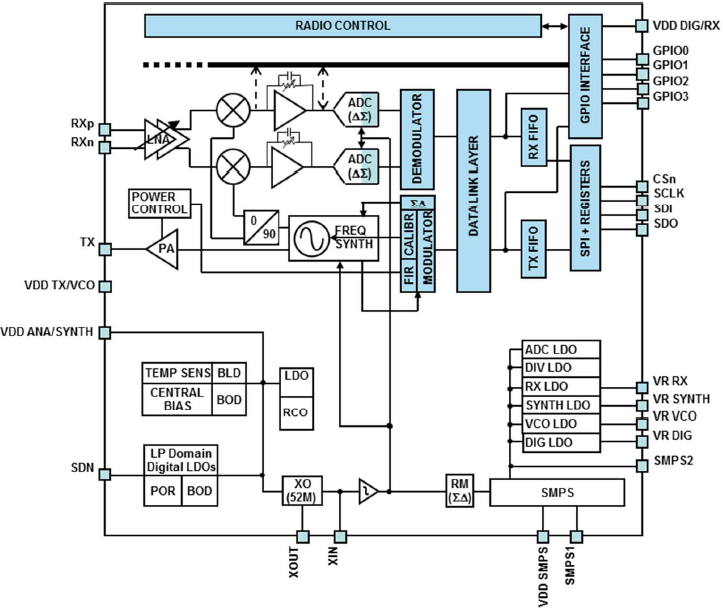
\includegraphics[scale=0.8]{images/spirit.png}
	\caption{Block diagram of SPIRIT}
\end{figure}
\subsection{SPIRIT1}
The SPIRIT1 is a very low-power RF transceiver, intended for RF wireless applications in the sub-1 GHz band. It is designed to operate both in the license-free ISM and SRD frequency bands at 169, 315, 433, 868, and 915 MHz, but can also be programmed to operate at other additional frequencies in the 300-348 MHz, 387-470 MHz, and 779-956 MHz bands. The air data rate is programmable from 1 to 500 kbps, and the SPIRIT1 can be used in systems with channel spacing of 12.5/25 kHz, complying with the EN 300 220 standard. It uses a very small number of discrete external components and integrates a configurable baseband modem, which supports data management, modulation, and demodulation.\\
The data management handles the data in the proprietary fully programmable packet format also allows the M-Bus standard compliance format (all performance classes). However, the SPIRIT1 can perform cyclic redundancy checks on the data as well as FEC encoding/decoding on the packets. The SPIRIT1 provides an optional automatic acknowledgement, retransmission, and timeout protocol engine in order to reduce overall system costs by handling all the high-speed link layer operations. Moreover, the SPIRIT1 supports an embedded CSMA/CA engine. An AES 128-bit encryption co-processor is available for secure data transfer. The SPIRIT1 fully supports antenna diversity with an integrated antenna switching control algorithm. The SPIRIT1 supports different modulation schemes: 2-FSK, GFSK, OOK, ASK, and MSK. Transmitted/received data bytes are buffered in two different three-level FIFOs (TX FIFO and RX FIFO), accessible via the SPI interface for host processing.
\subsection{SPIRIT1/SPIRIT2 Protocol Stack}
\begin{figure}[ht]
	\centering
	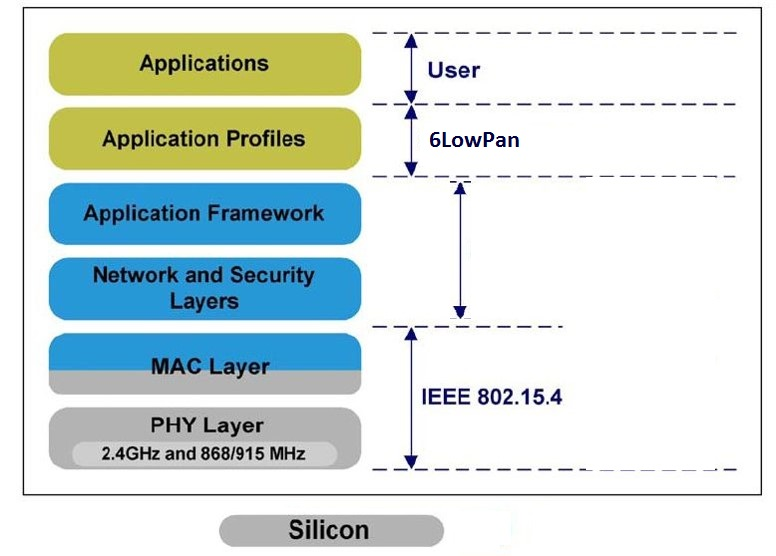
\includegraphics[scale=0.8]{images/protocol.png}
	\caption{spirit1/spirit2 protocol stack}
\end{figure}
Architecture of SPIRIT1 is similar to Spirit2 except it doesn’t follows IEEE 802.15.4 stack which is provided by the Linux kernel. If we talk about the protocols and Block Diagram then both are same but the only difference is that SPIRIT2 has 128 bits of FIFO register whereas SPIRIT1 has 96 bits of FIFO register.
\subsection{Pin Diagram of SPIRIT2}
\begin{figure}[ht]
	\centering
	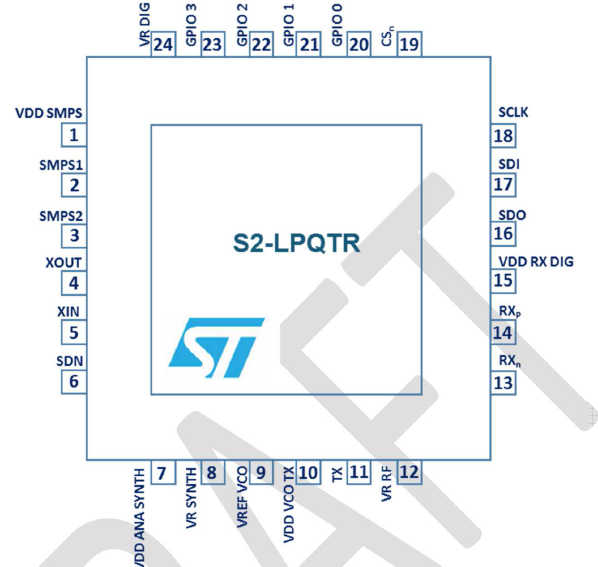
\includegraphics[scale=0.8]{images/pindiagram.png}
	\caption{Pin configuration of SPIRIT2}
\end{figure}
\subsection{Pin Description}
\begin{table}[ht]
	\centering
	\scalebox{0.8}{
	\begin{tabular}{|K{2cm} | K{4cm} | K{3cm} | K{10cm}|}
		\toprule
		\rowcolor{Gray}
		\textbf{N} & \textbf{Pin Name} & \textbf{Pin type} & \textbf{Description} \\
		\hline
		1 & VDD SMPS & POWER & \\
		\hline
		1 & VDD SMPS & POWER & 1.8 to 3.6 V analog power supply for SMPS only \\
		\hline
		2 & SMPS1 & Analog out & 1.1 to 1.8 V SMPS regulator output to be externally filtered \\
		\hline
		3 & SMPS2 & Analog in & 1.1 to 1.8 SMSP voltage input after LC filtering applied to SMPS1 output \\
		\hline 
		4 & XOUT & Analog out & Crystal oscillator output. connect to an external crystal or leave floating if driving the XIN pin with an external clock \\
		\hline 
		5 & XIN & Analog in & Crystal oscillator input. Connect to an external oscillator or to an external clock source \\
		\hline
		6 & SDN & Digital in & Shutdown input pin. SDN should be =  '0' in all modes but '1' in SHUTDOWN mode \\
		\hline
		7 & VDD ANA/SYNTH & Power & 1.8 to 3.6 V \\
		\hline 
		8 & VR SYNTH & Analog in/out & 1.2 V SYNTH-LDO output for decoupling \\
		\hline
		9 & VREF VCO & Analog out & 1.2 V VCO-LDO for decoupling \\
		\hline
		10 & VDD VCO/TX & Power & 1.8 V to 3.6 V power supply \\
		\hline
		11 & TX & RF output & RF output signal \\
		\hline
		12 & VR RF & Analog in/out & 1.2 V RX-LDO for decoupling \\
		\hline
		13 & RXn & RF in & Differential RF input signals for the LNA \\
		\hline
		14 & RXp & RF in & Differential RF input signals for the LNA \\
		\hline
		15 & VDD RX/DIG & Power & 1.8 to 3.6 V power supply \\
		\hline
		16 & SDO & Digital out & SPI slave data output \\
		\hline
		17 & SDI & Digital In & SPI slave data input \\
		\hline 
		18 & SCLK & Digital in & SPI slave clock input \\
		\hline 
		19 & CSn & Digital in & SPI chip select \\
		\hline
		20 & GPIO0 & Digital I/O & General purpose I/O \\
		\hline 
		21 & GPIO1 & Digital I/O & General purpose I/O \\
		\hline
		22 & GPIO2 & Digital I/O & General purpose I/O \\
		\hline
		23 & GPIO3 & Digital I/O & General purpose I/O \\
		\hline
		24 & VR DIG & Analog in/out & 1.2 V supply for decoupling\\
	\bottomrule
	\end{tabular}}
	\caption{SPIRIT pin description}
\end{table}
In this Report we mainly focused for the SPIRIT1 driver writing because I wrote the Driver for SPIRIT1, as we discussed in the previous section that the SPIRIT1 and SPIRIT2 architecture are same except the IEEE protocols.
\subsection{Operating Modes}
Several operating modes are defined for the SPIRIT:
\begin{itemize}
	\item Reset Mode
	\item Sleep Mode
	\item Standby Mode
	\item Ready Mode
	\item Lock Mode
	\item Shutdown Mode
\end{itemize}
The SPIRIT1 is provided with a built-in main controller which controls the switching between the two main operating modes: transmit (TX) and receive (RX). In shutdown condition (the SPIRIT1 can be switched on/off with the external pin SDN, all other functions/registers are available through the SPI interface and GPIOs), no internal supply is generated (in order to have minimum battery leakage), and hence, all stored data and configurations are lost. The GPIO and SPI ports during SHUTDOWN are in HiZ. From shutdown, the SPIRIT1 can be switched on from the SDN pin and goes into READY state, which is the default, where the reference signal from XO is available. From READY state, the SPIRIT1 can be moved to LOCK state to generate the high precision LO signal and/or TX or RX modes. Switching from RX to TX and vice versa can happen only by passing through the LOCK state. This operation is normally managed by radio control with a single user command (TX or RX). At the end of the operations above, the SPIRIT1 can return to its default state (READY) and can then be put into a sleeping condition (SLEEP state), having very low power consumption. If no timeout is required, the SPIRIT1 can be moved from READY to STANDBY state, which has the lowest possible current consumption while retaining FIFO, status and configuration registers. To manage the transitions towards and between these operating modes, the controller works as a state machine, whose state switching is driven by SPI commands. \\
\begin{figure}[ht]
	\centering
	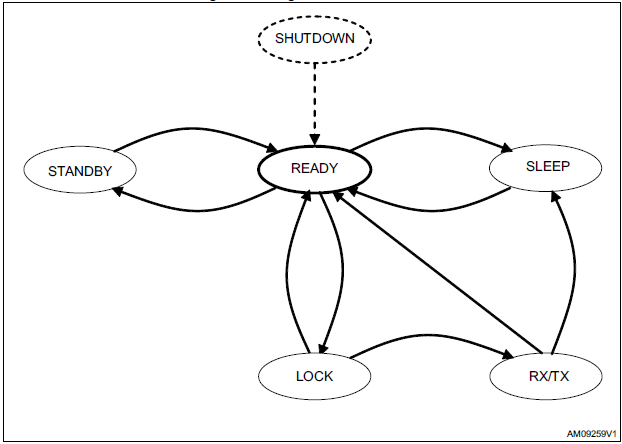
\includegraphics[scale=0.8]{images/modes.png}
	\caption{Operating modes of spirit}
\end{figure}
The SPIRIT1 radio control has three stable states (READY, STANDBY, LOCK) which may be defined stable, and they are accessed by the specific commands (respectively READY, STANDBY, and LOCKRX/LOCKTX), which can be left only if any other command is used. All other states are transient, which means that, in a typical configuration, the controller remains in those states, at most for any timeout timer duration. Also the READY and LOCK states behave as transients when they are not directly accessed with the specific commands (for example, when LOCK is temporarily used before reaching the TX or RX states).
\begin{figure}[ht]
	\centering
	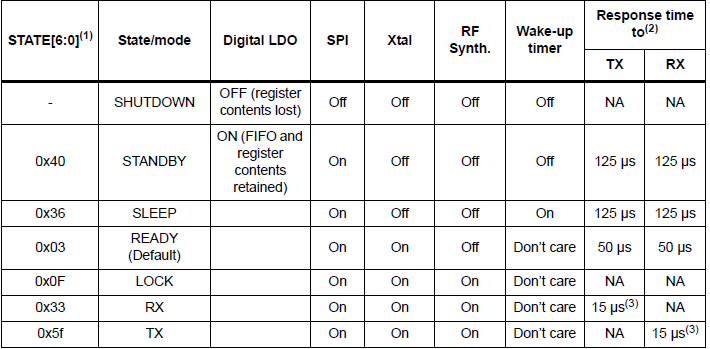
\includegraphics[scale=0.8]{images/table.png}
	\caption{Spirit opearting modes summary}
\end{figure}


